\documentclass[a4paper,12pt]{article} % тип документа

% report, book

% Рисунки
\usepackage{graphicx}
\usepackage{wrapfig}

\usepackage{hyperref}
\usepackage[rgb]{xcolor}
\hypersetup{				% Гиперссылки
    colorlinks=true,       	% false: ссылки в рамках
	urlcolor=blue          % на URL
}

%  Русский язык

\usepackage[T2A]{fontenc}			% кодировка
\usepackage[utf8]{inputenc}			% кодировка исходного текста
\usepackage[english,russian]{babel}	% локализация и переносы


% Математика
\usepackage{amsmath,amsfonts,amssymb,amsthm,mathtools} 


\usepackage{wasysym}

\author{Анна Назарчук Б02-109}
\title{1.2.3 Определение моментов инерции твердых тел с помощью трифилярного подвеса}
\date{}
\begin{document}
\maketitle
\section{Теоретические сведения}
Момент инерции твердого тела рассчитывается по формуле:
\begin{equation}
I = \int r^2dm
\end{equation}
Далеко не всегда удается вычислить момент инерции тела аналитически ввиду неоднородности или сложной формы, в таких случаях удобно сделать это экспериментально, например, с помощью трифилярного подвеса.
\begin{figure}[h!]
\begin{center}
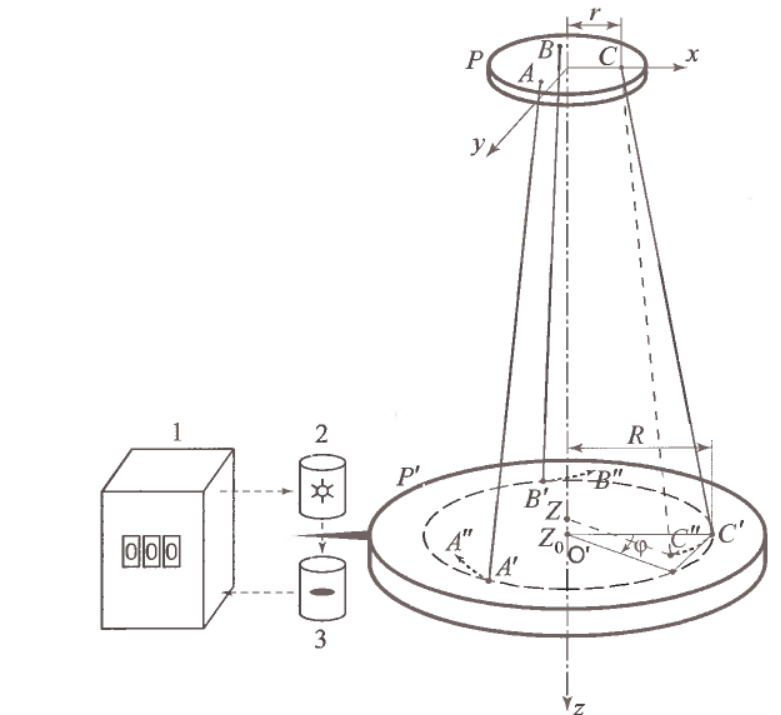
\includegraphics[width=0.7\textwidth]{Подвес}
\end{center}
\caption{Трифилярный подвес} \label{подвес}
\end{figure}
Устройство состоит из неподвижной платформы, вращающейся платформы, подвешенной на трех симметричных нитях.
Если пренебречь потерями энергии, то уравнение сохранения энергии при колебания:
\begin{equation}
\label{энергия}
\frac{I\dot{\varphi}^2}{2}+mg(z_0-z)=E,
\end{equation}
где $I$ - момент инерции платформы и тела, $z_0$ - координата по вертикали центра нижней платформы при равновесии, $z$ - координата аналогичной точки при повороте на угол $\phi$.
Из уравнения \ref{энергия} видно, что колебательное движение системы происходит благодаря силе тяжести. 

Рассмторим точку C на верхней платформе с координатами $(r, 0, 0)$ и точку $C''$, противоположную С при повороте на $\phi$, с координатами $(R\cos(\varphi), R\sin(\varphi)), z)$
Расстояние между нимим равно длине нити:
\begin{equation}
(R\cos(\phi)-r)^2+R^2\sin^2\phi+z^2=L^2
\end{equation}
Для малых углов:
\begin{equation}
z^2=L^2-R^2-r^2+2Rr\cos\varphi=z_0^2-2Rr(1-\cos\varphi)\approx z_0^2-Rr\varphi^2
\end{equation}
\begin{equation}
z \approx \sqrt{z_0^2-Rr\varphi^2}\approx z_0 \sqrt{1-\frac{Rr\varphi^2}{z_0^2}} \approx z_0- \frac{Rr\varphi^2}{2z_0}
\end{equation}
Подставив это в уравнение \ref{энергия}:
\begin{equation}
\frac{1}{2}I\dot{\varphi}+mg\frac{Rr}{2z_0}\varphi^2=E
\end{equation}
Откуда:
\begin{equation}
\varphi=\varphi_0\sin(\sqrt{\frac{mgRr}{Iz_0}}t+\Theta)
\end{equation}
Константны определяются начальными условиями, а период колебаний системы:
\begin{equation}
T=2\pi\sqrt{\frac{Iz_0}{mgRr}}
\end{equation}
Откуда не трудно определить выражние для момента инерции:
\begin{equation}
I=\frac{mgRrT^2}{2\pi^2z_0}
\end{equation}
Для краткости:
\begin{equation}
I=kmT^2
\end{equation}
Для постоянной k для данной установки:
\begin{equation}
k=I=\frac{gRr}{2\pi^2z_0}
\end{equation}

\section{Измерения и обработка данных}
\subsection{Измерения параметров установки}
Геометрические параметры установки представлены в таблице \ref{геом}, момент инерции пустой платформы (согласно таблице \ref{пустая}) равен:
\begin{equation}
I_{\text{платформы}} = 7.85 \pm 0.17 \text{г}\cdot \text{м}^2
\end{equation}
\begin{table} \label{геом} \caption{Геометрические параметры установки}
\begin{tabular}{|c|c|c|c|c|}
\hline 
$z_0$, мм& $R$, мм & r, мм & k, $\text{м}^2/\text{c}^2$ & $\sigma_k$, $\text{м}^2/\text{c}^2$ \\ 
\hline 
$2166.93 \pm 0.018$ & $115.4 \pm 0.5$ & $30.5 \pm 0.3$ & $0.40 \cdot 10^{-3}$ & $0.02 \cdot 10^{-3}$ \\ 
\hline 
\end{tabular} 
\end{table}

\begin{table} \label{пустая} \caption{Измерения момента инерции пустой платформы} \begin{tabular}{|c|c|c|c|c|c|c|} \hline N & $m_\text{груза}/\text{c}^2$, г & t, с & T, с & k, $\cdot 10^{-3}\text{м}^2/\text{c}^2$ & $m_\text{плат}, г$& $I_\text{тела}, \text{г}\cdot \text{м}^2$ \\ \hline 10 & 0 & 44 & 4.425 & 0.404 & 993 & 7.852 \\ \hline 10 & 0 & 44 & 4.422 & 0.404 & 993 & 7.841 \\ \hline 10 & 0 & 44 & 4.417 & 0.404 & 993 & 7.822 \\ \hline 11 & 0 & 48 & 4.423 & 0.404 & 993 & 7.846 \\ \hline 10 & 0 & 44 & 4.415 & 0.404 & 993 & 7.815 \\ \hline 10 & 0 & 44 & 4.411 & 0.404 & 993 & 7.801 \\ \hline 10 & 0 & 44 & 4.406 & 0.404 & 993 & 7.785 \\ \hline 10 & 0 & 44 & 4.402 & 0.404 & 993 & 7.772 \\ \hline \end{tabular} \end{table}


\subsection{Измерения моментов инерции разных тел}
\begin{table} \label{Диск} \caption{Измерение момента инерции диска} \begin{tabular}{|c|c|c|c|c|c|c|c|c|} \hline N & $m_\text{груза}$, г & t, с & T, с & k, $\cdot 10^{-3}\text{м}^2/\text{c}^2$ & $m_\text{плат}, г$ & $I_\text{системы}, \text{г}\cdot \text{м}^2$ &$I_\text{платформы}, \text{г}\cdot \text{м}^2$ & $I_\text{тела}, \text{г}\cdot \text{м}^2$ \\ \hline 10 & 590 & 39 & 3.958 & 0.404 & 993 & 10.013 & 7.817 & 2.197 \\ \hline 11 & 590 & 43 & 3.957 & 0.404 & 993 & 10.011 & 7.817 & 2.194 \\ \hline 10 & 590 & 39 & 3.953 & 0.404 & 993 & 9.988 & 7.817 & 2.171 \\ \hline 10 & 590 & 39 & 3.949 & 0.404 & 993 & 9.971 & 7.817 & 2.154 \\ \hline 10 & 590 & 39 & 3.953 & 0.404 & 993 & 9.99 & 7.817 & 2.173 \\ \hline 10 & 590 & 39 & 3.952 & 0.404 & 993 & 9.985 & 7.817 & 2.168 \\ \hline 10 & 590 & 39 & 3.95 & 0.404 & 993 & 9.975 & 7.817 & 2.159 \\ \hline 10 & 590 & 39 & 3.949 & 0.404 & 993 & 9.97 & 7.817 & 2.153 \\ \hline 10 & 590 & 39 & 3.948 & 0.404 & 993 & 9.963 & 7.817 & 2.146 \\ \hline 10 & 590 & 39 & 3.947 & 0.404 & 993 & 9.96 & 7.817 & 2.143 \\ \hline \end{tabular} \end{table}

\begin{table} \label{Цилиндр} \caption{Измерение момента инерции цилиндра} \begin{tabular}{|c|c|c|c|c|c|c|c|c|} \hline N & $m_\text{груза}$, г & t, с & T, с & k, $\cdot 10^{-3}\text{м}^2/\text{c}^2$ & $m_\text{плат}, г$ & $I_\text{системы}, \text{г}\cdot \text{м}^2$ &$I_\text{платформы}, \text{г}\cdot \text{м}^2$ & $I_\text{тела}, \text{г}\cdot \text{м}^2$ \\ \hline 13 & 772 & 54 & 4.226 & 0.404 & 993 & 12.728 & 7.817 & 4.911 \\ \hline 10 & 772 & 42 & 4.219 & 0.404 & 993 & 12.687 & 7.817 & 4.87 \\ \hline 10 & 772 & 42 & 4.217 & 0.404 & 993 & 12.67 & 7.817 & 4.854 \\ \hline 10 & 772 & 42 & 4.211 & 0.404 & 993 & 12.634 & 7.817 & 4.817 \\ \hline 10 & 772 & 42 & 4.208 & 0.404 & 993 & 12.622 & 7.817 & 4.805 \\ \hline 11 & 772 & 46 & 4.205 & 0.404 & 993 & 12.6 & 7.817 & 4.783 \\ \hline 11 & 772 & 46 & 4.202 & 0.404 & 993 & 12.584 & 7.817 & 4.767 \\ \hline 10 & 772 & 41 & 4.2 & 0.404 & 993 & 12.568 & 7.817 & 4.752 \\ \hline 10 & 772 & 41 & 4.2 & 0.404 & 993 & 12.57 & 7.817 & 4.753 \\ \hline 10 & 772 & 41 & 4.195 & 0.404 & 993 & 12.542 & 7.817 & 4.725 \\ \hline \end{tabular} \end{table}

\begin{table} \label{Параллелепипед} \caption{Измерение момента инерции параллелепипеда} \begin{tabular}{|c|c|c|c|c|c|c|c|c|} \hline N & $m_\text{груза}$, г & t, с & T, с & k, $\cdot 10^{-3}\text{м}^2/\text{c}^2$ & $m_\text{плат}, г$ & $I_\text{системы}, \text{г}\cdot \text{м}^2$ &$I_\text{платформы}, \text{г}\cdot \text{м}^2$ & $I_\text{тела}, \text{г}\cdot \text{м}^2$ \\  \hline 12 & 1077 & 45 & 3.789 & 0.404 & 993 & 12.003 & 7.817 & 4.186 \\ \hline 22 & 1077 & 83 & 3.786 & 0.404 & 993 & 11.979 & 7.817 & 4.162 \\ \hline 10 & 1077 & 37 & 3.783 & 0.404 & 993 & 11.961 & 7.817 & 4.145 \\ \hline 13 & 1077 & 49 & 3.782 & 0.404 & 993 & 11.957 & 7.817 & 4.14 \\ \hline 13 & 1077 & 49 & 3.776 & 0.404 & 993 & 11.92 & 7.817 & 4.103 \\ \hline 10 & 1077 & 37 & 3.78 & 0.404 & 993 & 11.945 & 7.817 & 4.128 \\ \hline 10 & 1077 & 37 & 3.777 & 0.404 & 993 & 11.925 & 7.817 & 4.108 \\ \hline 11 & 1077 & 41 & 3.778 & 0.404 & 993 & 11.928 & 7.817 & 4.111 \\ \hline 19 & 1077 & 72 & 3.794 & 0.404 & 993 & 12.031 & 7.817 & 4.214 \\ \hline 10 & 1077 & 37 & 3.791 & 0.404 & 993 & 12.012 & 7.817 & 4.195 \\ \hline \end{tabular} \end{table}


Измерения момента инерции диска представлены в таблице \ref{Диск}, согласно теоретическому расчету из геометрических размеров диска: $I_\text{диск}=2.11 \text{г}\cdot \text{м}^2$. Из полученных данных: $I_\text{диск}=2.17 \pm 0.07 \text{г}\cdot \text{м}^2$. Это подтверждает правильность метода измерения.

Измерения момента инерции цилиндра представлены в таблице \ref{Цилиндр}, согласно теоретическому расчету из геометрических размеров цилиндра: $I_\text{цилиндр}=4.64 \text{г}\cdot \text{м}^2$. Из полученных данных: $I_\text{цилиндр}=4.79 \pm 0.09 \text{г}\cdot \text{м}^2$. Это подтверждает правильность метода измерения.

Измерения момента инерции параллелепипеда представлены в таблице \ref{Параллелепипед}, согласно теоретическому расчету из геометрических размеров параллелепипеда: $I_\text{кубоид}=4.02 \text{г}\cdot \text{м}^2$. Из полученных данных: $I_\text{кубоид}=4.14 \pm 0.04 \text{г}\cdot \text{м}^2$. Это подтверждает правильность метода измерения.

\subsection{Проверка закона аддитивности момента инерции}
\begin{table} \label{Диск+цилиндр} \caption{Измерение момента инерции диска и цилиндра} \begin{tabular}{|c|c|c|c|c|c|c|c|c|} \hline N & $m_\text{груза}$, г & t, с & T, с & k, $\cdot 10^{-3}\text{м}^2/\text{c}^2$ & $m_\text{плат}, г$ & $I_\text{системы}, \text{г}\cdot \text{м}^2$ &$I_\text{платформы}, \text{г}\cdot \text{м}^2$ & $I_\text{тела}, \text{г}\cdot \text{м}^2$ \\  \hline 21 & 1362 & 83 & 3.953 & 0.404 & 993 & 14.86 & 7.817 & 7.043 \\ \hline 11 & 1362 & 43 & 3.91 & 0.404 & 993 & 14.813 & 7.817 & 6.996 \\ \hline 11 & 1362 & 43 & 3.943 & 0.404 & 993 & 14.786 & 7.817 & 6.969 \\ \hline 11 & 1362 & 43 & 3.91 & 0.404 & 993 & 14.76 & 7.817 & 6.944 \\ \hline 16 & 1362 & 62 & 3.936 & 0.404 & 993 & 14.734 & 7.817 & 6.917 \\ \hline 11 & 1362 & 43 & 3.934 & 0.404 & 993 & 14.712 & 7.817 & 6.895 \\ \hline 12 & 1362 & 47 & 3.932 & 0.404 & 993 & 14.7 & 7.817 & 6.883 \\ \hline 10 & 1362 & 39 & 3.929 & 0.404 & 993 & 14.677 & 7.817 & 6.861 \\ \hline 12 & 1362 & 47 & 3.91 & 0.404 & 993 & 14.678 & 7.817 & 6.861 \\ \hline 10 & 1362 & 39 & 3.928 & 0.404 & 993 & 14.672 & 7.817 & 6.855 \\ \hline \end{tabular} \end{table}

Согласно таблице \ref{Диск+цилиндр}: $I_\text{диск+цилиндр}=6.92 \pm 0.03 \text{г}\cdot \text{м}^2$. Согласно измереням моментов инерции тел по отдельности:
$I_\text{диск+цилиндр}=6.97 \pm 0.11 \text{г}\cdot \text{м}^2$.
Из чего следует справедливость закона аддитивности момента инерции.

\subsection{Измерение зависомости момента инерции диска от раздвижения его половинок}
\begin{table} \label{Половинки} \caption{Измерение момента инерции диска при движении половинок} \begin{tabular}{|c|c|c|c|c|c|c|c|c|c|} \hline N & $m_\text{груза}$, г & t, с & T, с & k, $\cdot 10^{-3}\text{м}^2$ & $m_\text{плат}, г$ & $I_\text{системы}, \text{г}\cdot \text{м}^2$ &$I_\text{платформы}, \text{г}\cdot \text{м}^2$ & $I_\text{тела}, \text{г}\cdot \text{м}^2$ & h, см \\ \hline 30 & 1528 & 91 & 3.061 & 0.404 & 993 & 9.536 & 7.817 & 1.72 & 0 \\ \hline 32 & 1528 & 98 & 3.067 & 0.404 & 993 & 9.575 & 7.817 & 1.758 & 0 \\ \hline 31 & 1528 & 95 & 3.074 & 0.404 & 993 & 9.616 & 7.817 & 1.8 & 1 \\ \hline 30 & 1528 & 93 & 3.12 & 0.404 & 993 & 9.907 & 7.817 & 2.09 & 1 \\ \hline 30 & 1528 & 94 & 3.157 & 0.404 & 993 & 10.147 & 7.817 & 2.33 & 2 \\ \hline 34 & 1528 & 109 & 3.21 & 0.404 & 993 & 10.486 & 7.817 & 2.669 & 2 \\ \hline 35 & 1528 & 114 & 3.275 & 0.404 & 993 & 10.916 & 7.817 & 3.099 & 3 \\ \hline 30 & 1528 & 100 & 3.338 & 0.404 & 993 & 11.338 & 7.817 & 3.521 & 3 \\ \hline 31 & 1528 & 106 & 3.429 & 0.404 & 993 & 11.97 & 7.817 & 4.154 & 4 \\ \hline \end{tabular} \end{table}
По данным из таблицы \ref{Половинки} построим график зависимости момента инерции диска от расстояния от каждой из половинок до центра платформы. График на рисунке \ref{график} 


\begin{figure}[h!]
\begin{center}
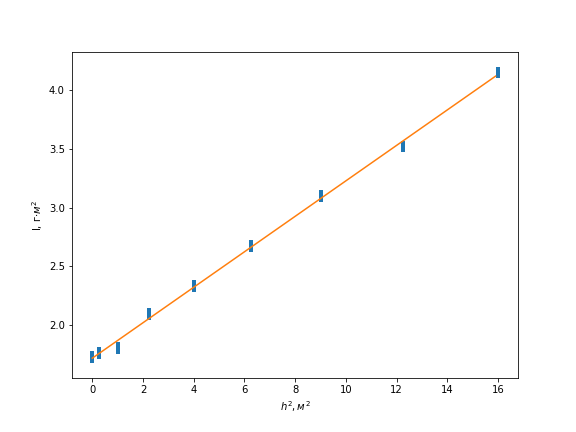
\includegraphics[width=\textwidth]{График}
\end{center}
\caption{График зависимости момента инерции диска от квадрата расстояния от каждой из половинок до центра платформы} \label{график}
\end{figure}


По наклону графика можно определить массу диска (в соотвествии в теоремой Гюйгенса-Штейнера): $m = 1.52 \pm 0.02 $кг, по отклонению найти момент инерции диска: $I = 1.69 \pm 0.02 \text{г}\cdot \text{м}^2$. Что согласуется с измеренной массой ($m = 1.53 \pm 0.02 $кг), теоретическим рассчетом момента инерции: $I = 1.53 \pm 0.02 \text{г}\cdot \text{м}^2$


\section{Вывод}
Измерены моменты инерции тел, результаты сравнены с теоретическими рассчетами, проверена справедливость аддидивности моента инерции и теорема Гюйгенса-Штейнера.
\end{document}